\chapter{Corridors at Scale and the v3 Corpus}
\label{ch:corpus_v3}

% ---------------------------------------------------------------------------
% Opens Part III. Planned sections (see the restructure plan, 2026-10-10):
%   - Repairing the grade field (below; moved from Ch. 5 on 2026-10-10)
%   - Scaling beyond a handful of corridors (below; moved from Ch. 5)
%   - Split corridor selection: 400-corridor pool, 389 built, 11 QA rejects;
%     populated control_eval; ood_grade on real mountain grade
%   - The v3 corpus build (50-100k scenarios), disk and cost, validation
% Sources: ROUTE_PIPELINE_NOTE.md Phases B-C, scripts/select_split_corridors.py,
% scripts/assign_split_corridors.py.
% ---------------------------------------------------------------------------

% TODO: chapter introduction.

\section{Repairing the grade field}
\label{sec:route_grade_fix}

The pipeline now checks the raw elevation first. A corridor on which more than 5\% of steps change by more than a metre is rejected, and the smoothing window is chosen only over the corridors that pass. \texttt{route\_line2} fails the check (\cref{sec:route_raw_qa}) and is removed, leaving four corridors. The window is then set to the narrowest value, 800\,m, at which the grade limit stops binding on every remaining corridor.

The grade limit was lowered from 4\% to 2.5\% at the same time, and its role changed. At 2.5\%, reaching the limit is itself a sign of an error in the data, and the fraction of a corridor that reaches it is reported. \Cref{tab:route_grade_stats} gives the resulting grade statistics, to be compared with \cref{tab:route_grade_stats_v2}.

\begin{table}[htbp]
    \centering
    \begin{tabular}{lcccc}
        \toprule
        Corridor & rms grade & 95th percentile & Maximum & Share at limit \\
        \midrule
        \texttt{route\_line0} (49\,km) & 0.86\% & 1.45\% & 2.50\% & 1.0\% \\
        \texttt{route\_line3} (29\,km) & 0.72\% & 1.25\% & 1.47\% & 0.0\% \\
        \texttt{route\_line4} (27\,km) & 0.39\% & 0.75\% & 1.23\% & 0.0\% \\
        \texttt{route\_line5} (22\,km) & 0.58\% & 0.87\% & 1.17\% & 0.0\% \\
        \bottomrule
    \end{tabular}
    \caption{Grade statistics for the four corridors that pass the raw-elevation check, with an 800\,m smoothing window and a 2.5\% grade limit.}
    \label{tab:route_grade_stats}
\end{table}

\texttt{route\_line0} still reaches the limit on 1.0\% of its length, in short runs with a median length of 135\,m. A real ruling grade is held for kilometres, so these runs are residual artifacts rather than terrain. They fall within the tolerance, and a filter on the minimum length of a grade excursion would be a more physical fix than further smoothing.

The effect on simulated trains is direct. In scenarios run on the old grade field, the fastest overspeed reached 67.8\,m/s, a freight train travelling at about 245\,km/h, and these extreme cases came from the false grades of \texttt{route\_line2}. On the corrected corridors the worst case falls to 25.7\,m/s. The share of scenarios exceeding the speed limit by more than 5\,m/s does not change: compared on the same four corridors, it is 13.3\% before and 13.5\% after. That shows it has a separate cause, which lies in how driving commands are generated rather than in the terrain. \Cref{ch:v3_sim} addresses it.

\begin{figure}[htbp]
    \centering
    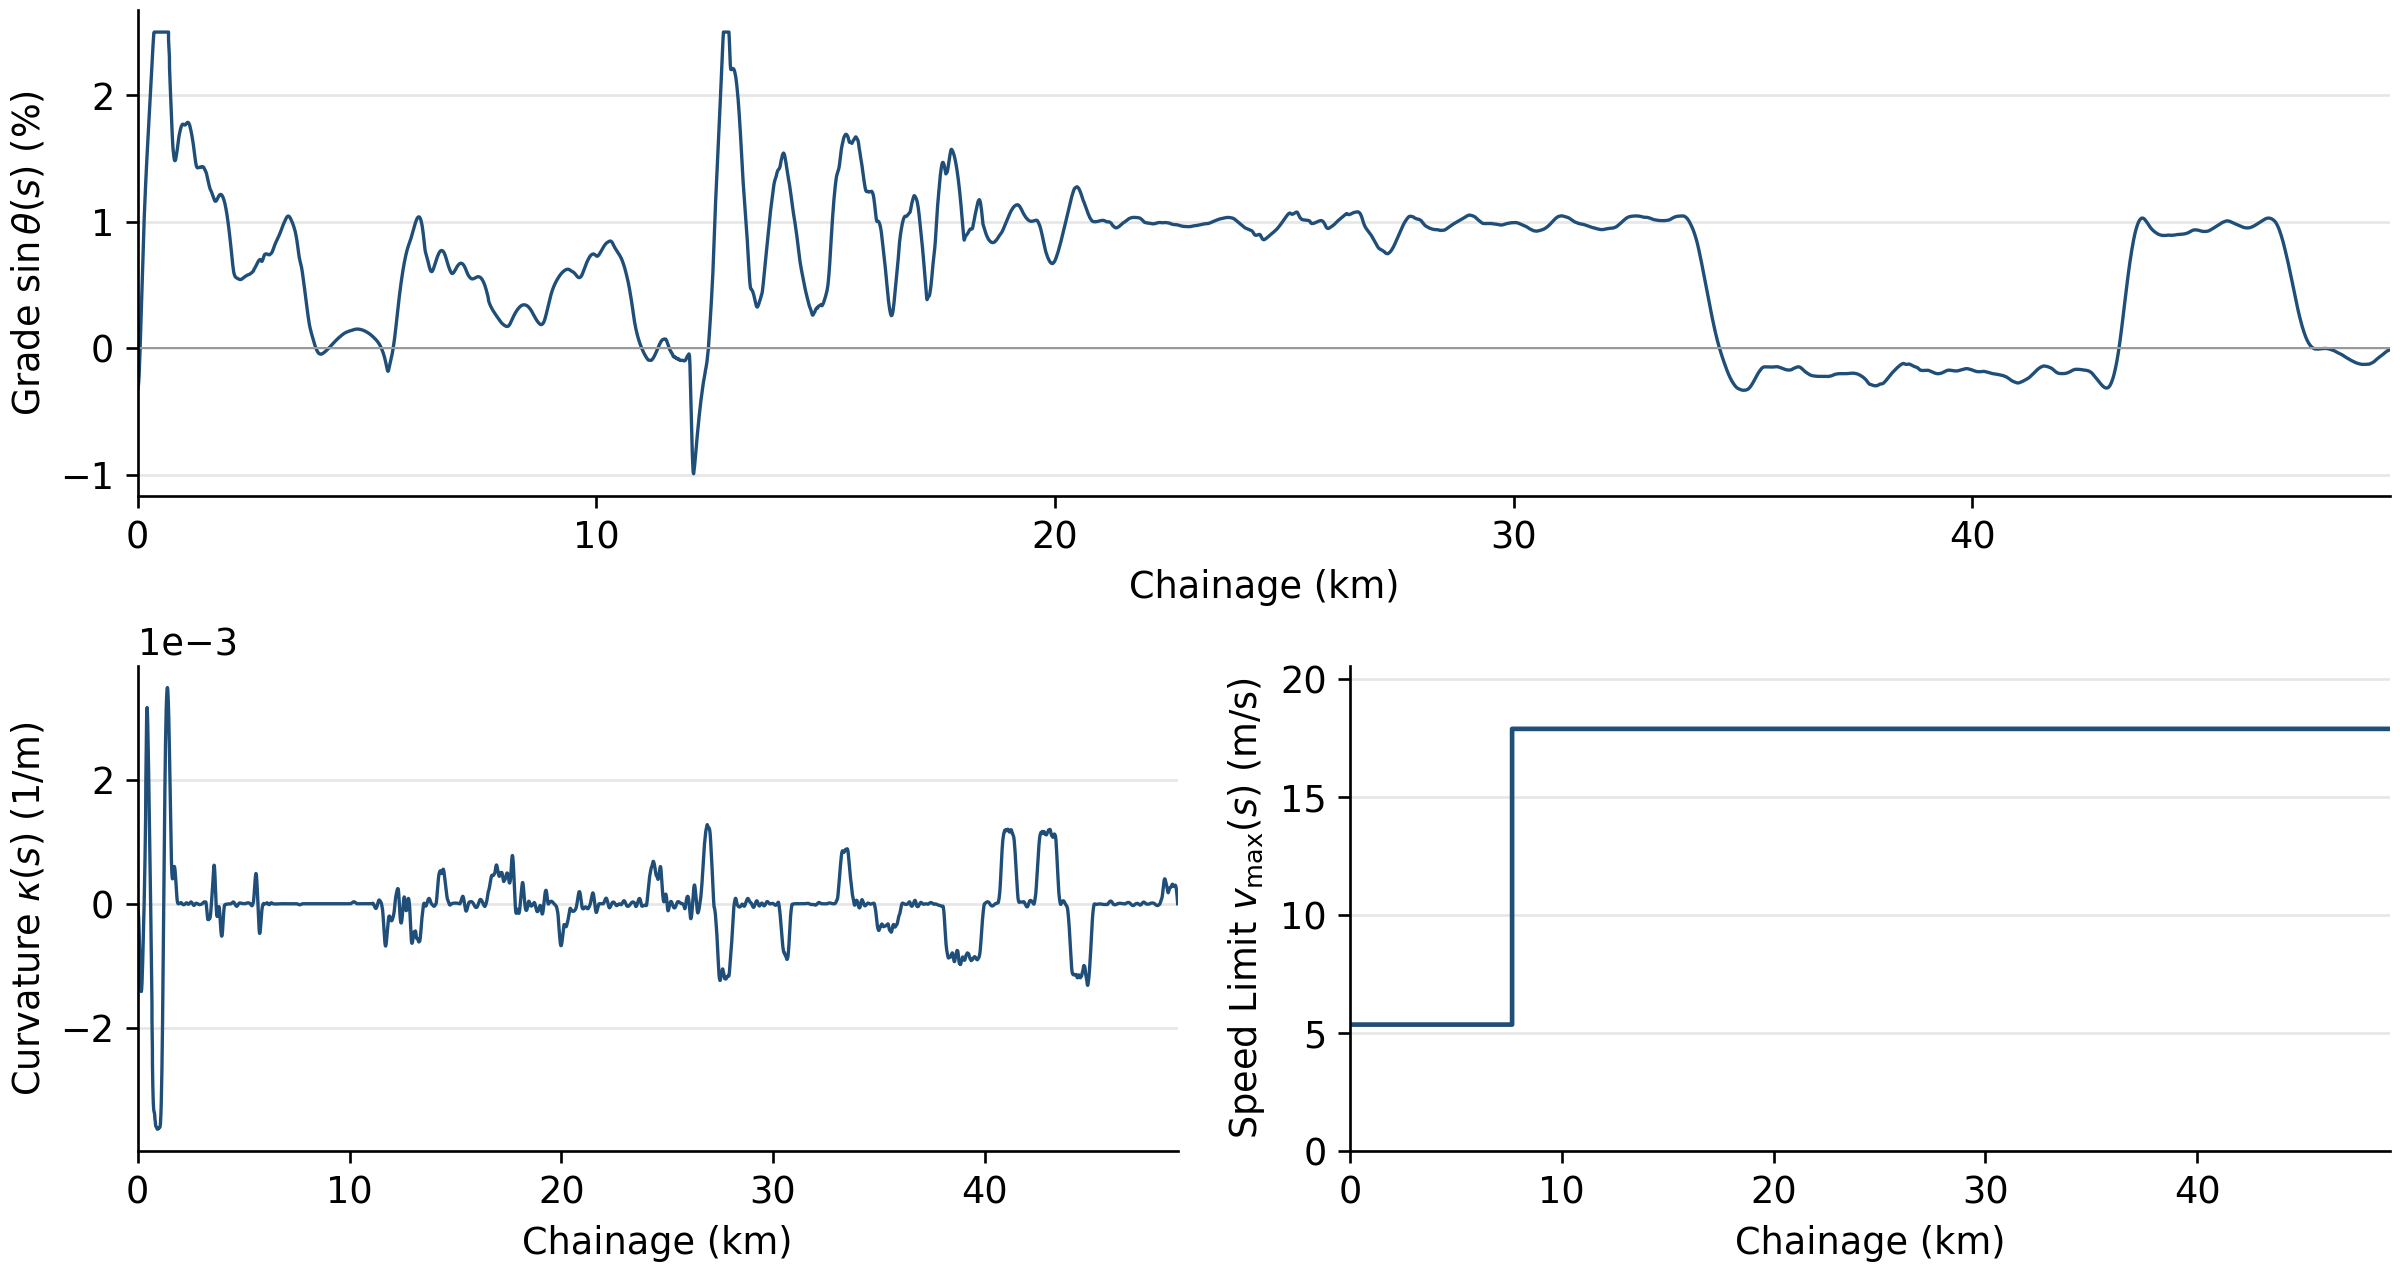
\includegraphics[width=0.92\textwidth]{thesis_imgs_7_15/route_generator/route_grade_curvature.png}
    \caption{The same fields as \cref{fig:route_grade_curvature}, for \texttt{route\_line0} after the raw-elevation check, with an 800\,m smoothing window and a 2.5\% grade limit. The urban approach over the first 20\,km is still the noisiest stretch, but the grade reaches the 2.5\% limit only in two short runs, near the start and near 12.7\,km, which are residual artifacts rather than terrain.}
    \label{fig:route_grade_curvature_v3}
\end{figure}

% TODO: the 2.5% clip was later split into a tripwire and a persistence
% filter, and tunnel flags are now recovered from the elevation itself
% (ROUTE_PIPELINE_NOTE.md, 2026-09-24). Write up here; the table and figure
% above describe the state before that change.

\section{Scaling beyond a handful of corridors}
\label{sec:route_scaling}

Five corridors are enough to build and test the pipeline, but not enough to support a strong claim about generalization to unseen routes, or to hold out a genuinely steep corridor for evaluation. The next step was therefore a larger, regional corridor set, and the pipeline was extended for it.

\subsection{The batch crawl}

For more than a few routes, a headless batch runner replaces the interactive application. It takes a curated list of seed points, runs the area-first acquisition and bounded outward crawl of \cref{sec:route_acquisition_stage1} from each, and merges the results into one dataset. Lines pulled from overlapping seeds are deduplicated by their shared map identifiers, keeping the longest version of any line pulled more than once, and the run caches each seed so it can resume after an interruption. Several measures keep individual queries to the Overpass service from timing out: service track and industrial, tourism, and military spurs are excluded at query time, the initial query for each seed is split into a grid of small requests, and every request retries with exponential backoff and can rotate across mirror servers.

A regional run of 22 seeds within 900\,km of Pueblo, Colorado, chosen to include steep crossings such as Raton Pass and Tennessee Pass, did not complete. It failed on five consecutive seeds with server-busy errors over 4.5 hours. The choice of server had been based on the time to answer a single test query, and a single query does not predict a sustained crawl: a server that answers one request quickly may throttle heavily once hundreds arrive. Retries and backoff do not help when the limit is the server's tolerance for the workload itself.

\subsection{The North American Rail Network}

The crawl was replaced by a different source of track geometry. The U.S. Department of Transportation's Bureau of Transportation Statistics publishes the North American Rail Network, a national dataset of rail line segments covering the United States, Canada, and Mexico, as a queryable feature service \cite{narn}. It removes the two hardest parts of the OSM path.

\begin{itemize}
    \item \textbf{Topology is explicit.} Every segment records the node it starts from and the node it ends at, so the network is already a graph. The OSM path had to reconstruct connectivity from fragment endpoints, which is where its gaps and branch-ordering problems came from.
    \item \textbf{Track is already classified.} Each of the 302,771 segments carries a network class assigned by the data's maintainers. Main-line track accounts for 95,936 segments; the rest are yard tracks, industrial leads, passing sidings, and out-of-service or abandoned line. The mainline filter that the OSM path approximated with tag rules is given directly.
\end{itemize}

It also carries attributes OSM did not reliably provide, including the owning railroad, the subdivision name, and the number of tracks, so corridors can be identified by their real names rather than by labels such as \texttt{route\_line2}. No rate limiting was observed. The full main-line network, 95,936 segments and 274,145\,km of track, was downloaded in 13.5 minutes.

The network does not include line speeds, so speed limits still come from OSM, queried per corridor rather than crawled.
% TODO: reconcile with ROUTE_PIPELINE_NOTE.md, which says derive_profile falls
% back to an FRA class from TRACKS and PASSNGR for NARN corridors (class 4
% single track, 5 for multiple tracks or passenger, 3 if unknown).
Elevation still comes from 3DEP. With the batched elevation queries of \cref{sec:route_elevation}, the rest of the pipeline is fast enough for the whole network: resampling, elevation, and profile derivation for all 274,145\,km at 10\,m spacing, about 27 million points, are projected to take roughly 36 minutes, almost all of it in elevation queries.
% TODO: check the 36-minute projection. ROUTE_PIPELINE_NOTE.md, "Elevation
% throughput does not reproduce", reports that the batch throughput was not
% reproduced in later runs.

\subsection{From network to corridors}

The network is a graph of segments averaging 2.9\,km in length, joined at 92,787 nodes, not a set of routes. The simulator needs continuous corridors with a single, increasing chainage, so a traversal stage was added before resampling. Network segments are adapted to the same way objects the OSM path produces, so the corridor walk of \cref{sec:route_acquisition_stage1} applies unchanged. Because connectivity is recorded in the data rather than inferred from endpoints, the gap-bridging and coordinate-fallback heuristics of the OSM path never fire.

Corridors are grown within each railroad subdivision, identified by owner and subdivision name together since names are reused across railroads. Long chains are cut at 60\,km and chains shorter than 15\,km are dropped. The traversal of the whole continent takes 93\,s and needs no network access. It yields 5,621 corridors (4,350 in the United States, 935 in Canada and 336 in Mexico), with a median length of 47.6\,km, retaining 248,892 of the 274,145\,km of main-line track. Corridors carry real identities, such as \texttt{bnsf\_raton\_p0\_56km} or \texttt{rrrr\_tennessee\_pass\_p0\_39km}, and corridor supply is no longer the constraint on the size of the evaluation splits.

% TODO: corridor selection for the splits (400-corridor pool, 389 built,
% 11 rejected by the elevation gate, 7 of them mountain corridors), the
% 3DEP coverage limit outside the US, and the measured mild bias of the gate
% against steep terrain. Sources: ROUTE_PIPELINE_NOTE.md. The assignment
% gave ood_corridor 25 corridors instead of 30 (and control_eval 25 instead
% of 20) until fixed on 2026-10-16; quote the sizes from a rerun.
